\scanpage{9}
\deleted{voisinage ouvert $W\ni t$, induisant ce qui est donné sur $W\cap U$. En fait, \deleted{d'après le} \inserted{si on dispose du} th. de Tate \deleted{\unsure{ceci}} \unsure{par suite} en inégales caractéristiques, on pourrait prouver}

b) Cas $S$ \deleted{normal} \inserted{géom. unib.}, $A_U$ muni d'une rigidification de Jacobi. On a donc un morphisme
\margin{\deleted{$\unsure{\ell}$}}
\diagram{\begin{tikzcd}U\arrow[r] & R\end{tikzcd}}
\margin{\figure{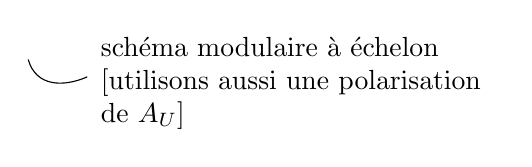
\begin{tikzpicture}\draw (0,.35) .. controls (.1,0) and (.45,0) .. (.75,.13);\node[anchor=west,text width=5cm] at (.8,.05) {schéma modulaire à \unsure{échelon} [utilisons aussi une polarisation de $A_U$]};\end{tikzpicture}}}
d'où par le \inserted{l'adhérence du} graphe un sous-schéma fermé $S'$ de $S\times R$. Le critère valuatif et le résultat de Raynaud dans le cas d'un trait \unsure{prouvent} que $S'\to S$ est propre. Il reste à prouver que c'est un isom [tout revient en effet, grâce à Tate, à prouver que $A_U$ se prolonge en $A$, quand $T_p(A_U)$ se prolonge en un $M$ -- cet $M$ étant en effet unique à iso unique près). Par le Main Theorem, on est ramené à prouver que \deleted{les pts de $S'$} \inserted{les fibres $S'_s$ sont \uline{discrètes}.} Introduisons le normalisé $S''$ de $S'$, qu'on suppose d'abord \uline{fini} sur $S'$. Alors le th. de Tate implique que le grpe $p$-divisible $T_p(A_{S''})$ \margin{\figure{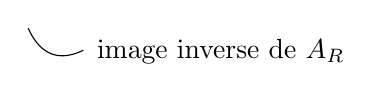
\begin{tikzpicture}\draw (0,.3) .. controls (.18,-.1) and (.45,-.1) .. (.7,.02);\node[anchor=west] at (.75,0) {image inverse de $A_R$};\end{tikzpicture}}} est l'image inverse de \deleted{$\unsure{T_p(A)}$} $M$. Donc la restriction de $A_{S''}\mid S''_s$, correspondant à un $T_p$ ``constant'', et $S''_s$ étant géom. connexe,
\margin{\diagram{\begin{tikzcd}[column sep=small,row sep=small]
 & S''\arrow[d]\arrow[r] & U''\arrow[d,phantom,"\unsure{\Vert|\wr}"]\\
R & S'\arrow[l]\arrow[d]\arrow[r] & U'\arrow[d,phantom,"\unsure{\Vert|\wr}"]\\
 & S\arrow[r] & U
\end{tikzcd}}}
\mspage{8}
